%\section{Modified Model with Length Control}
\section{Approach}
\label{sec:approach}

In this section, we will describe the model architecture used for our experiments
%and propose our reducing repetition method which is implemented by extending thebasic model.
and propose novel repetition reduction method, an extension to the basic model discussed in \secref{sec:basic}.

In summarization task, the input (source document) and
the output (target summary) are both sequences of elements.
Suppose the input is represented as
$\textbf{x} = (x_{1},x_{2},...,x_{m})$ and the output is represented as
$\textbf{y} = (y_{1}, y_{2},..., y_{n})$ ($m>n$),
the goal is to estimate the conditional probability
$p(\textbf{y}|\textbf{x})$:
\begin{equation}
p(\textbf{y} | \textbf{x}) \!=\! {\prod^T_{t} {p(y_{t} | y_{1}, y_{2},..., y_{t-1}, \textbf{x}})}
\end{equation}

Our goal is to model the above conditional probability in such a way that the generated summaries are not only fluent and consistent with source document, but also with a natural level of repetition similar to the reference summaries (results illustrated in \tabref{tab:eval_repe}). 
%We aim at getting the above conditional probability which can generate summaries without repetition.

\subsection{Basic CNN seq2seq Model}
\label{sec:basic}

\begin{figure}
    \centering
    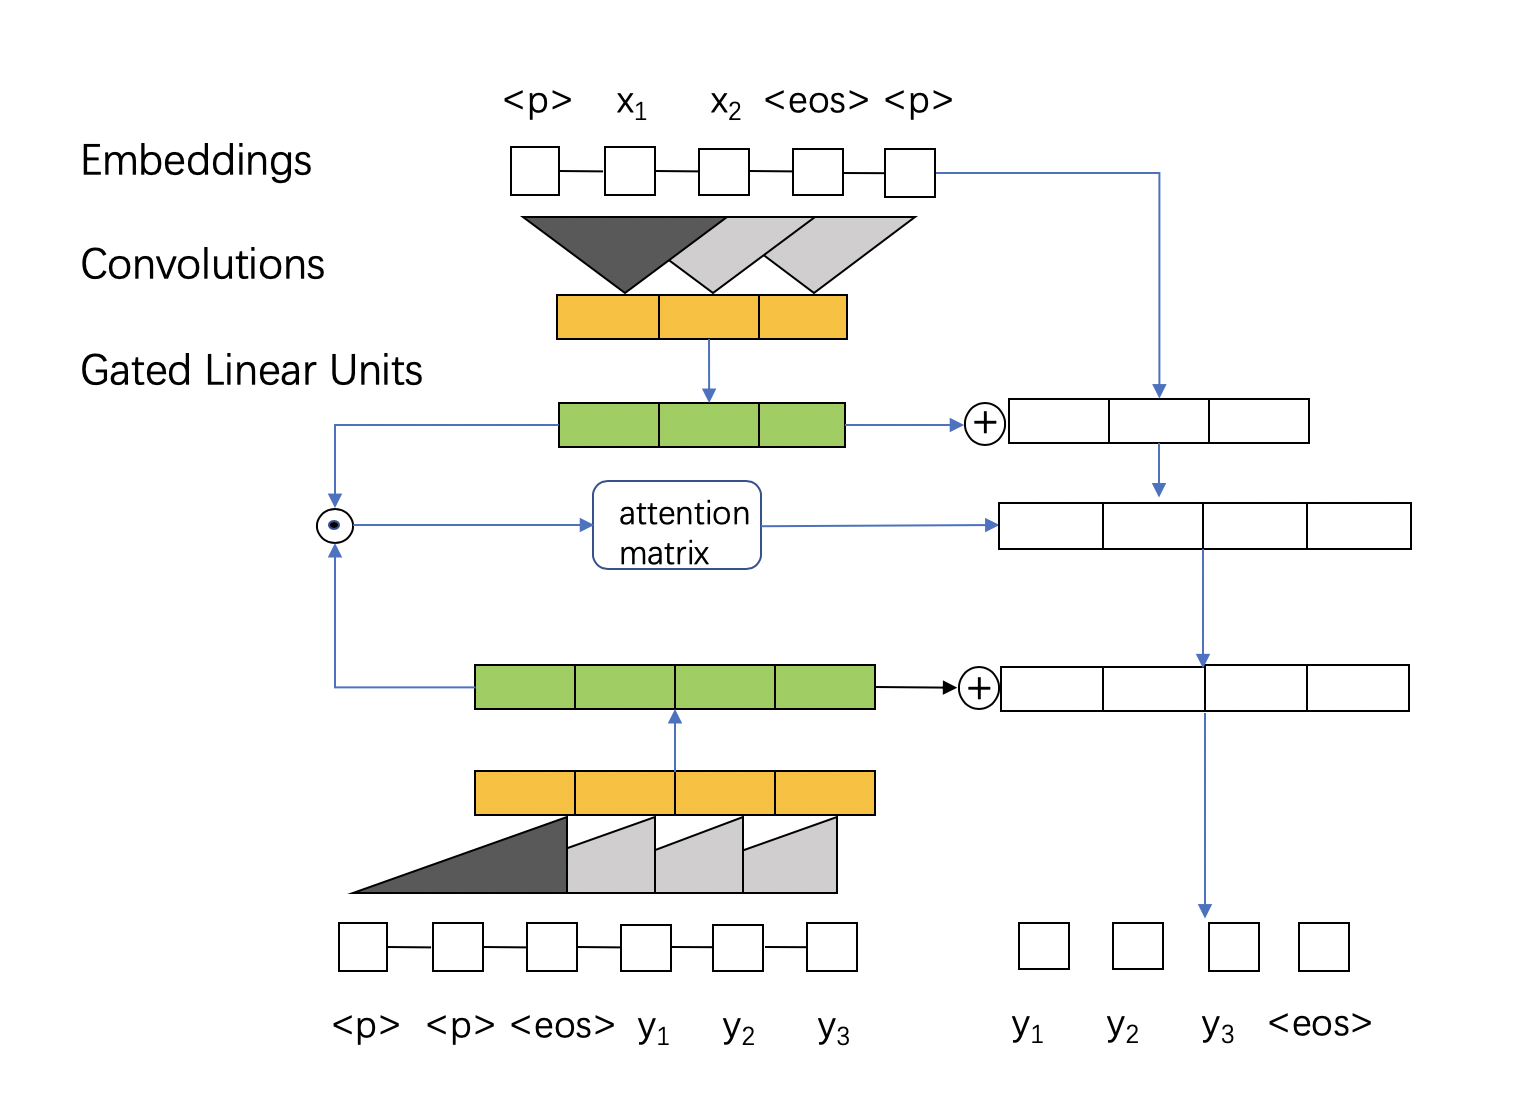
\includegraphics[width=0.8\linewidth]{basic_model.png}
    \caption{Convolutional seq2seq model. $\odot$ stands for inner product. $\oplus$ stands for element-wise addition.}
    \label{fig:basicModel}
\end{figure}

Our basic model includes multi-layer convolutional sequence to sequence networks \cite{gehring2017convs2s} and attention mechanism \footnote{\url{https://github.com/facebookresearch/fairseq-py}}, as is illustrated in \figref{fig:basicModel}. 

For CNN seq2seq models, we combine both word embeddings and position embeddings to obtain input element representations  $\mathbf{X} = (X_1,...,X_m)$ and output element representations $\mathbf{Y}=(Y_1,...,Y_n)$. We denote $\mathbf { z } ^ { l }$ and $\mathbf { h } ^ { l }$ respectively as convolutional output of the encoder and
decoder in the $l$-th layer, where $\mathbf { z } ^ { l } = \left( z _ { 1 } ^ { l } , \ldots , z _ { m } ^ { l } \right)$ and $\mathbf { h } ^ { l } = \left( h _ { 1 } ^ { l } , \ldots , h _ { n } ^ { l } \right)$. In each layer, GLU \cite{DauphinFAG17} is used as a non-linear gating mechanism and residual connections \cite{HeZRS16} ensure sufficient depth of networks.  
\begin{equation}
    h _ { i } ^ { l } = GLU \left( W ^ { l } \left[ h _ {i- \frac{1}{2}k } ^ { l - 1 } , \ldots , h _ { i+\frac{1}{2}k } ^ { l - 1 } \right] + b _ { w } ^ { l } \right) + h _ { i } ^ { l - 1 }
\end{equation}
In this way, convolutional blocks connect up successive layers ($h^{l-1}$ and $h^{l}$). Next, we compute the probability distribution for the next word using the top decoder output and softmax:
\begin{equation}
    p \left( y _ { i + 1 } | y _ { 1 } , \ldots , y _ { i } , \mathbf { x } \right) = \operatorname { softmax } \left( W _ { o } h _ { i } ^ { L } + b _ { o } \right) \in \mathbb { R } ^ { T }
\end{equation}

For each decoder layer, a multi-step attention mechanism is introduced to integrate encoder information. We compute decoder state summary $d_{i}^{l}$ via
\begin{equation}
    d _ { i } ^ { l } = W _ { d } ^ { l } h _ { i } ^ { l } + b _ { d } ^ { l } + Y _ { i }
\end{equation}

The inner product between decoder state summary and encoder outputs is used 
to measure the affinity. The conditional input to the current 
decoder layer is a weighted sum of both encoder states and input element representations.
\begin{equation}\label{eq:a}
    a _ { i j } ^ { l } = \frac { \exp \left( d _ { i } ^ { l } \cdot z _ { j } ^ { u } \right) } { \sum _ { t = 1 } ^ { m } \exp \left( d _ { i } ^ { l } \cdot z _ { t } ^ { u } \right) }
\end{equation}
\begin{equation}\label{eq:c}
    c _ { i } ^ { l } = \sum _ { j = 1 } ^ { m } a _ { i j } ^ { l } \left( z _ { j } ^ { u } + X_j \right)
\end{equation}
where $z_{j}^{u}$ is the encoder output of last layer $u$.  
Finally, $c _ { i } ^ { l }$ is added to $h_{i}^{l}$ as the input for the next decoder layer.

\subsection{Attention Filter Mechanism(ATTF)}
\label{sec:attf}

\begin{figure*}[th]
	\centering
	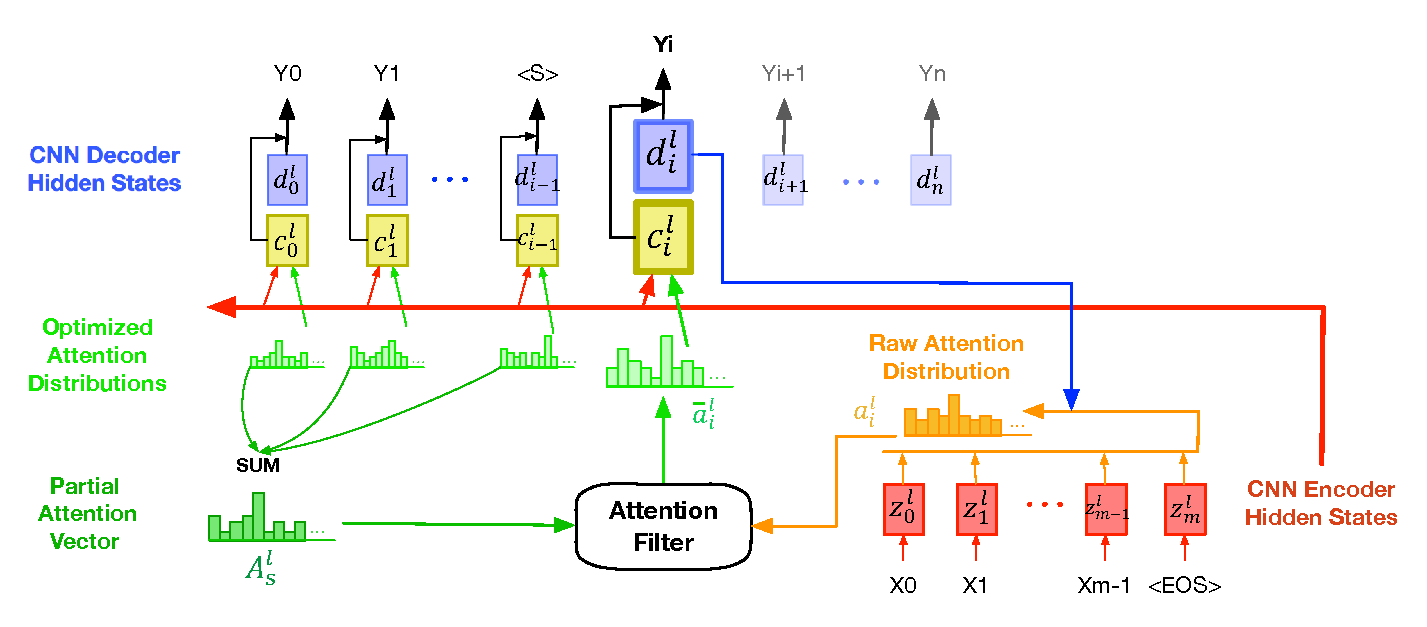
\epsfig{file=model.eps, width=2\columnwidth}
	\caption{Overview of proposed model, which shows how Attention Filter Mechanism (ATTF) works when decoding $Y_i$.}
	\label{fig:model_main}
\end{figure*}


\label{sec:attnf}
%We propose an attention filter mechanism based on basic model
We propose an attention filter mechanism as an novel extension to the basic model introduced above,
which can record previously attended locations 
%previously POIs 
in source document in a direct manner and generate summaries 
%without repetition
with a natural level of repetition. 
This method aims to relieve the repetition problem caused by 
decoders attending to the same POI%section
in source document.

In this mechanism, source document and summary are respectively split into 
\textit{sections} and \textit{segments} by punctuation $<$s$>$.
$\mathbf{u}=(u_{0},u_{1},...,u_{M})$ 
and $\mathbf{v}=(v_{0},v_{1},...,v_{N})$
denote the positions of $<$s$>$ in source document and summary.
Both $u_{0}$ and $v_{0}$ are $0$.
%Source document $\mathbf{U}=(U_{0},U_{1},...,U_{M-1})$ 
%and summary $\mathbf{V}=(V_{0},V_{1},...,V_{N-1})$ are represented in the form of sections and.
Therefore, we can represent source document as $\mathbf{U}=(U_{0},U_{1},...,U_{M-1})$ in the form of \textit{sections}. Similarly, for summaries, we have $\mathbf{V}=(V_{0},V_{1},...,V_{N-1})$.

Let $w$ denote the number of unique tokens in the source document.
We define \textit{segment attention vector} in the $l$-th layer as 
$A^{l} = (A_{0}^{l}, A_{1}^{l},..., A_{N}^{l})$, 
where $A_s^l\subset \mathbb{R}^{w}$ is a vector representing 
segment attention distribution, of the $s$-th \textit{segment},
over tokens in source document. Sum up attention score vectors 
of each position in the $s$-th \textit{segment}:
%which is the sum of attention distributions over each section in summary:

\begin{equation}
    A_{s}^{l} = \sum_{i=v_{s-1}}^{v_{s}}a_{i}^{l}
\end{equation}

where $a_i^l$ is also a $w$-dimensional vector that records 
the attention scores of the $i$-th token in the summary over 
tokens in source document. In other words, $ A_{s}^{l}$ 
measures the relevance between tokens of source document and 
the $s$-th \textit{segment} $V_s^{l}$.
%where vector $A_{n}^{l}$ is the partial attention distribution over the words in source document. 
%It represents the degree of relevance between source document and the $n$-th section in summary.
We set $A_{0}^{l}$ as zero vector, because nothing is attended before generating the first \textit{segment}. 


To find most attended \textit{sections}, 
we sort the elements inside the filter vector, 
$A_{s}^{l}$, in descending order, 
and record the top $k$ elements' positions in 
source document as: 
\begin{equation}
    \mathbf{p}=(p_{0},...,p_{k})
\end{equation}
where $k = v_{s} - v_{s-1}$.
%To get the attended sections of document, we sort elements $A_{nj}^{l}$ in descending order, and record the positions a
%in decreasing order, and record the position
%$\mathbf{p}=(p_{0},...,p_{k})$, of 
%top $k$ elements in source document, where $k = v_{n} - v_{n-1}$. 
%The higher value of $A_{nj}^{l}$ means that the $j$-th words of source document has been attended. 
%We find out which section of these top $k$ elements belong to by $\mathbf{p}$ and $\mathbf{u}$.
Next, we locate these elements in the source document and 
find out the \textit{sections} that they belong to. 
Therefore, each section has a attended position set $P_{U_{t}}$. 
If the size of an attended position set $P_{U_{t}}$ is larger than
$sz$, a predefined constant,
%\footnote{$sz$ is a constant. 
%We set $sz$ as 3, because nearly 90 percent
%of sections with lengt$>=$3.}, 
the \textit{section $U_{t}$} should not be attended again. 
We use $\bar{U}$ to express this kind of section. 
%the \textit{section $U_{t}$} can be seen as the POI by $V_s^{l}$. 

We construct two multi-hot vectors $g_{s}$ and $g^{'}_{s}$ for each \textit{segment} $s$.
The dimensions of them are the
same as $A_{s}^{l}$. For $g_{s}$, we set elements on the position of $\bar{U}$ to 0, and other
%same as $A_{s}^{l}$. For $g_{s}$, we set elements on the position of POIs to 0, and other
positions to 1. $g^{'}_{s}$ is the flipped version of $g_{s}$. 
%The filter on $a_{ij}^{l}$ in Equation (\ref{eq:a} is to minimize elements of POIs:
The filter on $a_{ij}^{l}$ in Equation (\ref{eq:a} is given as:

\begin{equation}
    e_{s} = \min \limits_{A_{s}}\left(\frac{A_{sj}^{l}}{v_{s+1}-v_{s}}\right)
\end{equation}
\begin{equation}
    \bar{a}_{ij}^{l} = a_{ij}^{l}\prod_{q=0}^{s}g_{q} + e_{s}g^{'}_{s}
    %\bar{a_{ij}}^{l} = a_{ij}^{l}\prod_{q=0}^{n}s_{q} + \min\frac{A_{n}^{l}}{v_{n}-v_{n-1}}t_{n}
\end{equation}

where $s$ is the maximum value in 
$\mathbf{v}$ that is smaller than $i$.  
%\XS{Hard to understand this definition of ``n''. And ``n'' is already used to be the size of output in Section 2.1}
The Equation (\ref{eq:c}) now changes to:
\begin{equation}
    c _ { i } ^ { l } = \sum _ { j = 1 } ^ { m } \bar{a} _ { i j } ^ { l } \left( z _ { j } ^ { u } + x_j \right)
\end{equation}

%We pick $K$ sections with highest attention which is calculated by:
%\begin{equation}
%    A_{nj}^{l} = \sum^{P}A_{nj}^{l}
%\end{equation}

%This method find out the attended location in source document directly and accurately.
%Then it filters out attention of the attended location from the attention distribution. 
In this way, our attention filter is capable of comprehending the attention history i
in a precise and direct manner. 
%The previous approaches revise attention scores
%through decoder hidden state. They can not locate POIs exactly.
%The coverage model which gets the sum of all previous attention can 
%bring attention noise, especially in the long summary.
Because of using segment attention and revising attention score of attended POIs directly,
it optimizes the 
attention distribution between encoder states and decoder states in such a way that
the alignment relationship between source document and summary is enhanced, and noise for attention from encoder outputs reduced. 
Thus, attention filter mechanism helps avoid repeatedly attending to similar POIs, and therefore avoid repetition in summary generation.


\subsection{Sentence-level Backtracking Decoder (SBD) at Test Time}

As mentioned in \secref{sec:intro}, another reason that gives rise to repetition is repetitive sentences and paragraphs in source documents.
%To handle the repetition caused by repetitive sentences in source document(\tabref{tab:src_rep}),
To tackle this problem, we propose a sentence-level backtracking decoder during testing.

At test time, we prevent our decoder from generating similar sentences more 
than once via backtracking. 
Specifically, every time the decoder is to generate a sentence $S$
that is similar to one that already exists in previous generations, 
we get position $p$ at the end of last sentence and backtrack to  
the beginning of summary.
In the proccess of generating new summary, 
we do not generate the same word as the first word in $S$ at step $p$.
Other two methods of backtracking are compared in \secref{sec:eval}.
One(SBD-b1) is to regenerate this sentence from the end of last sentence.
The other(SBD-b2) is backtracking to the most adjust decoder state 
that all of generated sequences in beam size
before this state are the same.
To determine whether two sentences, 
$p$ and $q$, are similar, we define $sim(p, q)$ as a boolean function:
\begin{equation}\label{eq:s}
    sim(p,q) = o > n\text{ or }o > \frac{1}{2}\cdot l
\end{equation}
where $o$ denotes the number of overlapped words in $p$ and $q$, 
$l$ is the minimum of the lengths of $p$ and $q$, and $n$ is a constant. 
$sim(p,q)=1$ means the two sentence are similar.
%We set $n$ as 5, because the number of overlapped words in target summaries
%is less than 5 percent.
%\KW{maybe mention c=5 in experiment settings, the notation in the formula is not clean enough but i don't know how to revise it}

This method does not attempt to impact the process of beam search in the middle of a sentence so that we are free of grammatical and factual errors compared with our \textbf{TRI} baseline.
Besides, it potentially brings about a more informative summary by 
giving more chances to other candidate sentences while reducing repetition.
%, which we validate in relevant experiments
%(\tabref{tab:src_rep}, \figref{fig:attn_map3}).
